\section*{Appendix}

\subsection*{Diagramme}
In diesem Abschnitt werden manche der verwendeten Abbildungen in gr��erer Version aufgef�hrt.

%Kapitel2
\begin{figure}[H]
    \centering
    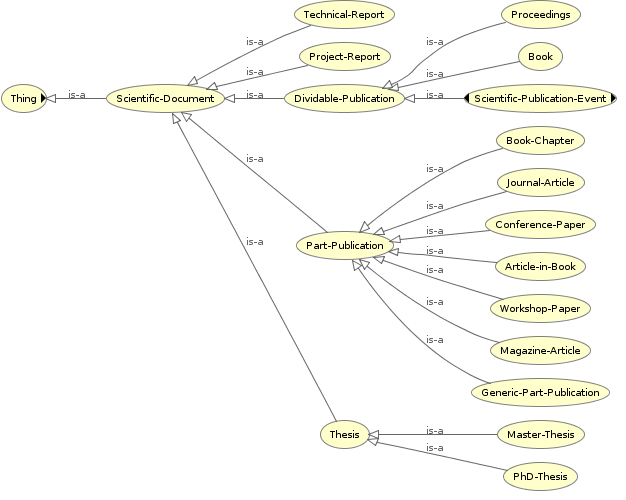
\includegraphics[angle=90,scale=0.65]{../deps/ontology_of_science_scientificdoc_owlviz.png}
    \caption{Ontology of Science. Die Klasse \textit{Scientific Document}}
    \label{fig:scientificdociBig}
\end{figure}

%Kapitel 3
\begin{figure}[H]
        \centering
        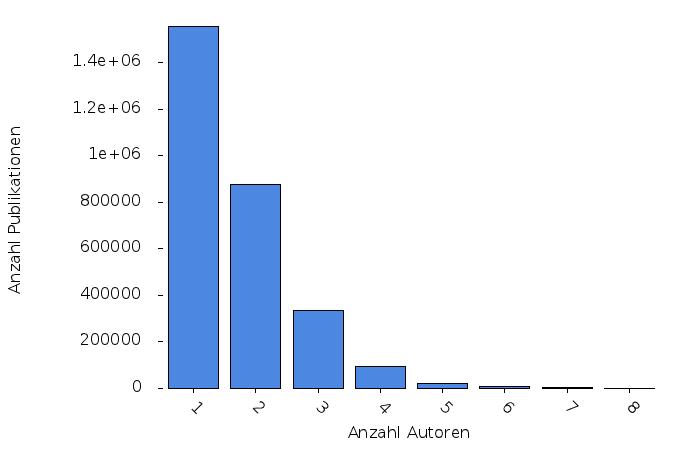
\includegraphics[scale=0.5]{../data/statistics/authorFreq.png}
        \caption{Autorenverteilung}
        \label{fig:authorFreqBig}
\end{figure}

\begin{figure}[H]
        \centering
        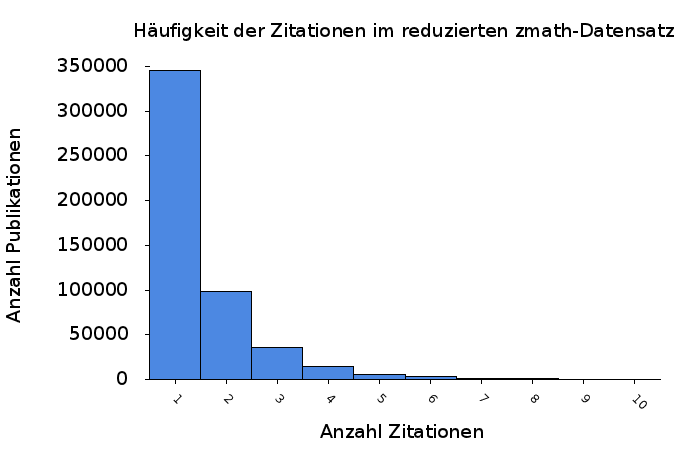
\includegraphics[scale=.5]{../data/statistics/citationFreq.png}
        \caption{Zitationsverteilung}
        \label{fig:citationFreqBig}
\end{figure}

\begin{figure}[H]
        \centering
        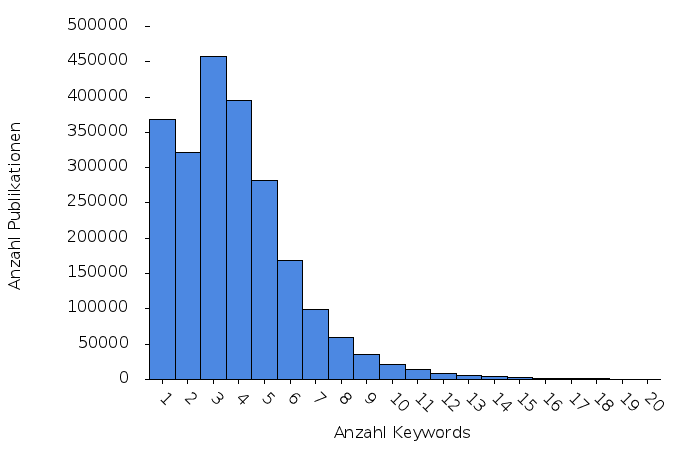
\includegraphics[scale=.5]{../data/statistics/keyWordFreq.png}
        \caption{Keywordverteilung}
        \label{fig:keywordFreqBig}
\end{figure}

\begin{figure}[H]
        \centering
        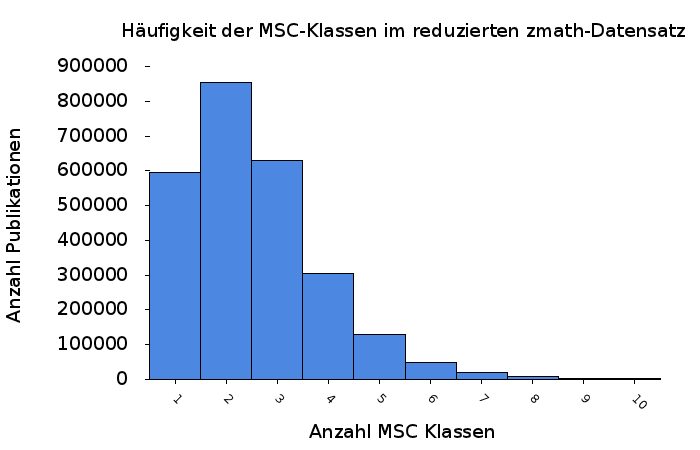
\includegraphics[scale=.5]{../data/statistics/mscClassFreq.png}
        \caption{Verteilung der MSC-Klassen}
        \label{fig:mscClassFreqBig}
\end{figure}

%Kapitel 4
\begin{figure}[H]
        \centering
        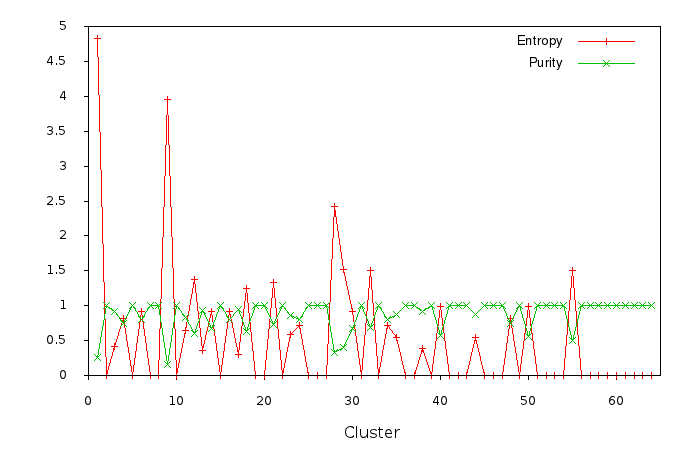
\includegraphics[scale=0.5]{../evaluation/diss_true/crankPurityEntropy.png}
        \caption{Purity und Entropy des \textit{pam}-Clustering von \textit{C-Rank}}
        \label{fig:crankEntPurBig}
\end{figure}


\begin{figure}[H]
        \centering
        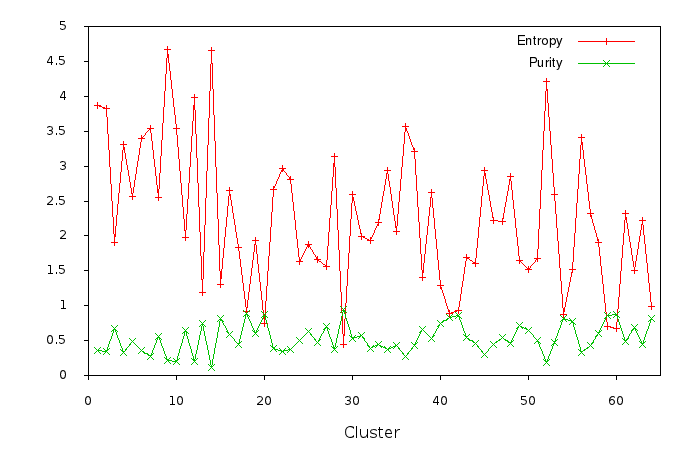
\includegraphics[scale=0.5]{../evaluation/diss_true/p1PurityEntropy.png}
        \caption{Purity und Entropy des \textit{pam}-Clustering von Gewichtung 1}
        \label{fig:p1EntPurBig}
\end{figure}

\begin{figure}[H]
        \centering
        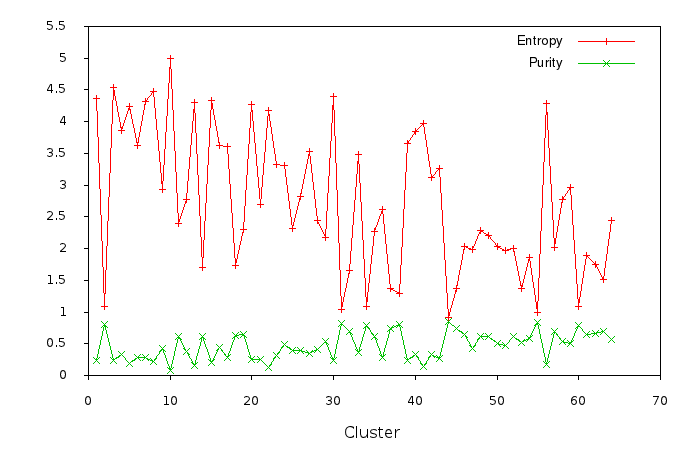
\includegraphics[scale=0.5]{../evaluation/diss_true/p2PurityEntropy.png}
        \caption{Purity und Entropy des \textit{pam}-Clustering von Gewichtung 2}
        \label{fig:p2EntPurBig}
\end{figure}

\begin{figure}[H]
        \centering
        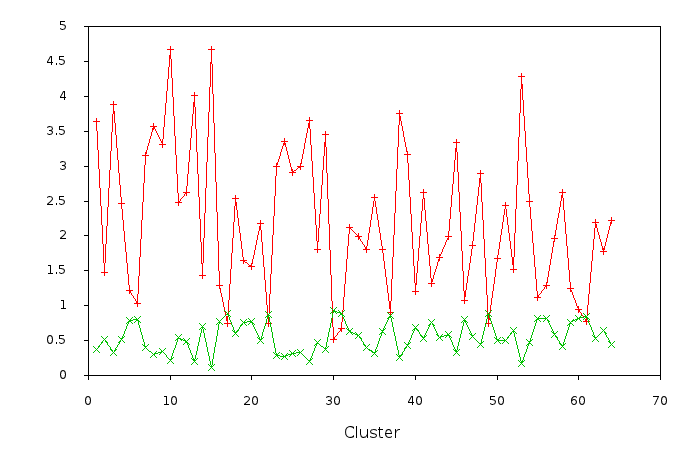
\includegraphics[scale=0.5]{../evaluation/diss_true/p3PurityEntropy.png}
        \caption{Purity und Entropy des \textit{pam}-Clustering von Gewichtung 3}
        \label{fig:p3EntPurBig}
\end{figure}

\subsection*{Ergebnisse des \textit{pam} Clustering}

\begin{longtable}[H]{| l | l | l | l | l |}
%\begin{tabular}{| l | l | l | l | l |}
		\multicolumn{2}{l}{\textbf{C-Rank}} \\
		\hline
        \textbf{ClusterID} & \textbf{\# Publikationen} & \textbf{Entropy} & \textbf{Purity} & \textbf{Gr��te MSC Klasse}\\
	    \hline
        $1$ & $2587$ & $4.8228$ & $0.2613$ & 11-XX : 676 Pubs\\
        $2$ & $10$ & 0 & 1.0 & 11-XX : $10$ Pubs\\
        $3$ & $12$ & 0.413816850304 & 0.916666666667 & 11-XX : $11$ Pubs\\
        $4$ & $4$ & 0.811278124459 & 0.75 & 16-XX : $3$ Pubs\\
        $5$ & $9$ & 0 & 1.0 & 11-XX : $9$ Pubs\\
        $6$ & $10$ & 0.921928094887 & 0.8 & 20-XX : $8$ Pubs\\
        $7$ & $16$ & 0 & 1.0 & 11-XX : $16$ Pubs\\
        $8$ & $16$ & 0 & 1.0 & 11-XX : $16$ Pubs\\
        $9$ & $26$ & 3.95006375644 & 0.153846153846 & 46-XX : $4$ Pubs\\
        $10$ & $9$ & 0 & 1.0 & 47-XX : $9$ Pubs\\
        $11$ & $6$ & 0.650022421648 & 0.833333333333 & 57-XX : $5$ Pubs\\
        $12$ & $5$ & 1.37095059445 & 0.6 & 16-XX : $3$ Pubs\\
        $13$ & $15$ & 0.353359335021 & 0.933333333333 & 11-XX : $14$ Pubs\\
        $14$ & $6$ & 0.918295834054 & 0.666666666667 & 11-XX : $4$ Pubs\\
        $15$ & $15$ & 0 & 1.0 & 11-XX : $15$ Pubs\\
        $16$ & $10$ & 0.921928094887 & 0.8 & 06-XX : $8$ Pubs\\
        $17$ & $19$ & 0.297472248919 & 0.947368421053 & 11-XX : $18$ Pubs\\
        $18$ & $11$ & 1.24067053168 & 0.636363636364 & 76-XX : $7$ Pubs\\
        $19$ & $3$ & 0 & 1.0 & 54-XX : $3$ Pubs\\
        $20$ & $7$ & 0 & 1.0 & 11-XX : $7$ Pubs\\
        $21$ & $22$ & 1.33420945945 & 0.727272727273 & 05-XX : $16$ Pubs\\
        $22$ & $5$ & 0 & 1.0 & 11-XX : $5$ Pubs\\
        $23$ & $7$ & 0.591672778582 & 0.857142857143 & 11-XX : 6.0 Pubs\\
        $24$ & $5$ & 0.721928094887 & 0.8 & 47-XX : $4$  Pubs\\
        $25$ & $13$ & 0 & 1.0 & 11-XX : $13$  Pubs\\
        $26$ & $3$ & 0 & 1.0 & 03-XX : $3$  Pubs\\
        $27$ & $4$ & 0 & 1.0 & 11-XX : $4$  Pubs\\
        $28$ & $12$ & 2.41829583405 & 0.333333333333 & 68-XX : $4$  Pubs\\
        $29$ & $5$ & 1.52192809489 & 0.4 & 91-XX : $2$  Pubs\\
        $30$ & $3$ & 0.918295834054 & 0.666666666667 & 17-XX : $2$  Pubs\\
        $31$ & $4$ & 0 & 1.0 & 62-XX : $4$  Pubs\\
        $32$ & $13$ & 1.5058762556 & 0.692307692308 & 74-XX : $9$  Pubs\\
        $33$ & $6$ & 0 & 1.0 & 11-XX : $6$  Pubs\\
        $34$ & $5$ & 0.721928094887 & 0.8 & 35-XX : $4$  Pubs\\
        $35$ & $8$ & 0.5435644432 & 0.875 & 11-XX : $7$  Pubs\\
        $36$ & $12$ & 0 & 1.0 & 11-XX : $12$  Pubs\\
        $37$ & $7$ & 0 & 1.0 & 11-XX : $7$  Pubs\\
        $38$ & $13$ & 0.391243563629 & 0.923076923077 & 11-XX : $12$  Pubs\\
        $39$ & $14$ & 0 & 1.0 & 11-XX : $14$  Pubs\\
        $40$ & $7$ & 0.985228136034 & 0.571428571429 & 68-XX : $4$  Pubs\\
        $41$ & $8$ & 0 & 1.0 & 11-XX : $8$  Pubs\\
        $42$ & $7$ & 0 & 1.0 & 11-XX : $7$  Pubs\\
        $43$ & $3$ & 0 & 1.0 & 03-XX : $3$  Pubs\\
        $44$ & $8$ & 0.5435644432 & 0.875 & 54-XX : $7$ Pubs\\
        $45$ & $4$ & 0 & 1.0 & 54-XX : $4$  Pubs\\
        $46$ & $6$ & 0 & 1.0 & 54-XX : $6$  Pubs\\
        $47$ & $11$ & 0 & 1.0 & 54-XX : $11$  Pubs\\
        $48$ & $4$ & 0.811278124459 & 0.75 & 26-XX : $3$ Pubs\\
        $49$ & $7$ & 0 & 1.0 & 11-XX : $7$  Pubs\\
        $50$ & $9$ & 0.991076059838 & 0.555555555556 & 11-XX : $5$  Pubs\\
        $51$ & $3$ & 0 & 1.0 & 16-XX : $3$  Pubs\\
        $52$ & $4$ & 0 & 1.0 & 11-XX : $4$  Pubs\\
        $53$ & $6$ & 0 & 1.0 & 11-XX : $6$  Pubs\\
        $54$ & $6$ & 0 & 1.0 & 11-XX : $6$  Pubs\\
        $55$ & $4$ & 1.5 & 0.5 & 49-XX : $2$  Pubs\\
        $56$ & $2$ & 0 & 1.0 & 11-XX : $2$  Pubs\\
        $57$ & $9$ & 0 & 1.0 & 11-XX : $9$  Pubs\\
        $58$ & $8$ & 0 & 1.0 & 53-XX : $8$  Pubs\\
        $59$ & $3$ & 0 & 1.0 & 54-XX : $3$  Pubs\\
        $60$ & $4$ & 0 & 1.0 & 11-XX : $4$  Pubs\\
        $61$ & $4$ & 0 & 1.0 & 11-XX : $4$  Pubs\\
        $62$ & $5$ & 0 & 1.0 & 00-XX : $5$  Pubs\\
        $63$ & $4$ & 0 & 1.0 & 30-XX : $4$  Pubs\\
        $64$ & $2$ & 0 & 1.0 & 11-XX : $2$  Pubs\\
        \hline
%\end{tabular}
\end{longtable}


\begin{longtable}[H]{| l | l | l | l | l |}
%\begin{tabular}{| l | l | l | l | l |}
		\multicolumn{2}{l}{\textbf{Gewichtung 1}} \\
		\hline
        \textbf{ClusterID} & \textbf{\# Publikationen} & \textbf{Entropy} & \textbf{Purity} & \textbf{Gr��te MSC Klasse}\\
	    \hline
        $1$ & $93$ & 3.86357242492 & 0.354838709677 & 11-XX: $33$  Pubs\\
        $2$ & $76$ & 3.83219711006 & 0.342105263158 & 11-XX: $26$  Pubs\\
        $3$ & $27$ & 1.90086342713 & 0.666666666667 & 65-XX:  $18$  Pubs\\
        $4$ & $46$ & 3.31219729491 & 0.326086956522 & 11-XX:  $15$  Pubs\\
        $5$ & $43$ & 2.557472165 & 0.488372093023 & 62-XX:  $21$  Pubs\\
        $6$ & $67$ & 3.39482356379 & 0.358208955224 & 11-XX:  $24$  Pubs\\
        $7$ & $36$ & 3.53462596246 & 0.277777777778 & 11-XX:  10.0  Pubs\\
        $8$ & $48$ & 2.54347077087 & 0.5625 & 00-XX:  $27$  Pubs\\
        $9$ & $160$ & 4.6664715524 & 0.2125 & 74-XX:  $34$  Pubs\\
        $10$ & $41$ & 3.53245636015 & 0.19512195122 & 16-XX: $8$  Pubs\\
        $11$ & $31$ & 1.97230721691 & 0.645161290323 & 20-XX: $20$  Pubs\\
        $12$ & $55$ & 3.980027026 & 0.2 & 11-XX:  $11$  Pubs\\
        $13$ & $16$ & 1.18627812446 & 0.75 & 16-XX:  $12$  Pubs\\
        $14$ & $87$ & 4.65818035335 & 0.114942528736 & 11-XX:  $10$  Pubs\\
        $15$ & $76$ & 1.30167674047 & 0.815789473684 & 60-XX:  $62$  Pubs\\
        $16$ & $181$ & 2.64529145205 & 0.585635359116 & 54-XX:  $106$  Pubs\\
        $17$ & $9$ & 1.83659166811 & 0.444444444444 & 11-XX:  $4$  Pubs\\
        $18$ & $123$ & 0.91217229883 & 0.886178861789 & 11-XX:  $109$  Pubs\\
        $19$ & $35$ & 1.93242157887 & 0.6 & 11-XX:  $21$  Pubs\\
        $20$ & $31$ & 0.748326550438 & 0.870967741935 & 11-XX:  $27$  Pubs\\
        $21$ & $65$ & 2.66336672653 & 0.384615384615 & 11-XX:  $25$  Pubs\\
        $22$ & $29$ & 2.96732853225 & 0.344827586207 & 11-XX:  $10$  Pubs\\
        $23$ & $37$ & 2.80640986878 & 0.378378378378 & 90-XX:  $14$  Pubs\\
        $24$ & $22$ & 1.63880671841 & 0.5 & 03-XX:  $11$  Pubs\\
        $25$ & $43$ & 1.87634324156 & 0.627906976744 & 42-XX:  $27$  Pubs\\
        $26$ & $47$ & 1.66484165241 & 0.468085106383 & 05-XX:  $22$  Pubs\\
        $27$ & $23$ & 1.56704021693 & 0.695652173913 & 11-XX:  $16$  Pubs\\
        $28$ & $68$ & 3.14131342143 & 0.367647058824 & 11-XX:  $25$  Pubs\\
        $29$ & $106$ & 0.441263671757 & 0.943396226415 & 11-XX:  $100$  Pubs\\
        $30$ & $40$ & 2.59708926037 & 0.525 & 11-XX:  $21$  Pubs\\
        $31$ & $19$ & 1.99484144464 & 0.578947368421 & 30-XX:  $11$  Pubs\\
        $32$ & $116$ & 1.93417135648 & 0.387931034483 & 46-XX:  $45$  Pubs\\
        $33$ & $18$ & 2.19161164175 & 0.444444444444 & 40-XX:  $8$  Pubs\\
        $34$ & $43$ & 2.93279310473 & 0.372093023256 & 11-XX:  $16$  Pubs\\
        $35$ & $44$ & 2.06117328526 & 0.431818181818 & 11-XX:  $19$  Pubs\\
        $36$ & $47$ & 3.56276988699 & 0.276595744681 & 11-XX:  $13$  Pubs\\
        $37$ & $66$ & 3.21492588746 & 0.424242424242 & 11-XX:  $28$  Pubs\\
        $38$ & $29$ & 1.39866157341 & 0.655172413793 & 17-XX:  $19$  Pubs\\
        $39$ & $92$ & 2.62007519126 & 0.532608695652 & 20-XX:  $49$  Pubs\\
        $40$ & $20$ & 1.29176014818 & 0.75 & 11-XX:  $15$  Pubs\\
        $41$ & $36$ & 0.893213741153 & 0.833333333333 & 35-XX:  $30$  Pubs\\
        $42$ & $81$ & 0.934853722782 & 0.864197530864 & 11-XX:  $70$  Pubs\\
        $43$ & $11$ & 1.68581570915 & 0.545454545455 & 18-XX:  $6$  Pubs\\
        $44$ & $37$ & 1.6017001683 & 0.459459459459 & 11-XX:  $17$  Pubs\\
        $45$ & $23$ & 2.94067621881 & 0.304347826087 & 11-XX:  $7$  Pubs\\
        $46$ & $49$ & 2.22476095411 & 0.448979591837 & 53-XX:  $22$  Pubs\\
        $47$ & $35$ & 2.20584692466 & 0.542857142857 & 11-XX:  $19$  Pubs\\
        $48$ & $61$ & 2.85163539057 & 0.459016393443 & 34-XX:  $28$  Pubs\\
        $49$ & $28$ & 1.64883485428 & 0.714285714286 & 11-XX:  $20$  Pubs\\
        $50$ & $57$ & 1.51617521702 & 0.649122807018 & 30-XX:  $37$  Pubs\\
        $51$ & $20$ & 1.67838982472 & 0.5 & 11-XX:  $10$  Pubs\\
        $52$ & $49$ & 4.2053496395 & 0.183673469388 & 76-XX:  $9$  Pubs\\
        $53$ & $45$ & 2.59646612559 & 0.466666666667 & 11-XX:  $21$  Pubs\\
        $54$ & $16$ & 0.86839272901 & 0.8125 & 11-XX:  $13$  Pubs\\
        $55$ & $76$ & 1.51331136325 & 0.776315789474 & 54-XX:  $59$  Pubs\\
        $56$ & $54$ & 3.41003244966 & 0.333333333333 & 11-XX:  $18$  Pubs\\
        $57$ & $26$ & 2.31375711026 & 0.423076923077 & 14-XX:  $11$  Pubs\\
        $58$ & $23$ & 1.91235080775 & 0.608695652174 & 11-XX:  $14$  Pubs\\
        $59$ & $15$ & 0.699842839886 & 0.866666666667 & 11-XX: $13$  Pubs\\
        $60$ & $16$ & 0.6685644432 & 0.875 & 11-XX:  $14$  Pubs\\
        $61$ & $33$ & 2.31712139209 & 0.484848484848 & 53-XX:  $16$  Pubs\\
        $62$ & $13$ & 1.5058762556 & 0.692307692308 & 74-XX:  $9$  Pubs\\
        $63$ & $20$ & 2.21497982052 & 0.45 & 45-XX:  $9$  Pubs\\
        $64$ & $16$ & 0.99339272901 & 0.8125 & 11-XX: $13$  Pubs\\
        \hline
%\end{tabular}
\end{longtable}

\begin{longtable}[H]{| l | l | l | l | l |}
%\begin{tabular}{| l | l | l | l | l |}
		\multicolumn{2}{l}{\textbf{Gewichtung 2}} \\
		\hline
        \textbf{ClusterID} & \textbf{\# Publikationen} & \textbf{Entropy} & \textbf{Purity} & \textbf{Gr��te MSC Klasse}\\
	    \hline
        1 & 99 & 4.36493171599 & 0.242424242424 & 11-XX :  24 Pubs\\
        2 & 21 & 1.08341893224 & 0.809523809524 & 11-XX :  17 Pubs\\
        3 & 117 & 4.53502174265 & 0.239316239316 & 11-XX :  28 Pubs\\
        4 & 102 & 3.85837209718 & 0.323529411765 & 20-XX :  33 Pubs\\
        5 & 93 & 4.23908882481 & 0.182795698925 & 11-XX :  17 Pubs\\
        6 & 32 & 3.62377812446 & 0.28125 & 11-XX :  9 Pubs\\
        7 & 100 & 4.31499006222 & 0.28 & 11-XX :  28 Pubs\\
        8 & 82 & 4.48279975475 & 0.219512195122 & 11-XX :  18 Pubs\\
        9 & 37 & 2.93203005464 & 0.432432432432 & 00-XX :  16 Pubs\\
        10 & 109 & 5.0013546233 & 0.0825688073394 & 11-XX :  9 Pubs\\
        11 & 66 & 2.39031219218 & 0.621212121212 & 11-XX :  41 Pubs\\
        12 & 35 & 2.76828183555 & 0.371428571429 & 20-XX :  13 Pubs\\
        13 & 50 & 4.3014678802 & 0.16 & 11-XX :  8 Pubs\\
        14 & 13 & 1.70043971814 & 0.615384615385 & 14-XX :  8 Pubs\\
        15 & 93 & 4.34071843442 & 0.204301075269 & 11-XX :  19 Pubs\\
        16 & 173 & 3.62662932431 & 0.439306358382 & 54-XX :  76 Pubs\\
        17 & 81 & 3.6133683379 & 0.283950617284 & 11-XX :  23 Pubs\\
        18 & 51 & 1.72694924493 & 0.627450980392 & 74-XX :  32 Pubs\\
        19 & 54 & 2.3052617041 & 0.648148148148 & 11-XX :  35 Pubs\\
        20 & 99 & 4.27549700681 & 0.252525252525 & 54-XX :  25 Pubs\\
        21 & 12 & 2.68872187554 & 0.25 & 14-XX :  3 Pubs\\
        22 & 78 & 4.16992802748 & 0.128205128205 & 46-XX :  10 Pubs\\
        23 & 35 & 3.32433549455 & 0.314285714286 & 11-XX :  11 Pubs\\
        24 & 75 & 3.3086261967 & 0.493333333333 & 11-XX :  37 Pubs\\
        25 & 10 & 2.32192809489 & 0.4 & 20-XX :  4 Pubs\\
        26 & 65 & 2.82198365611 & 0.4 & 11-XX :  26 Pubs\\
        27 & 34 & 3.52806431158 & 0.352941176471 & 11-XX :  12 Pubs\\
        28 & 37 & 2.4469398681 & 0.405405405405 & 05-XX :  15 Pubs\\
        29 & 17 & 2.1739731346 & 0.529411764706 & 11-XX :  9 Pubs\\
        30 & 126 & 4.40001315996 & 0.238095238095 & 11-XX :  30 Pubs\\
        31 & 27 & 1.04720247957 & 0.814814814815 & 11-XX :  22 Pubs\\
        32 & 23 & 1.65399673867 & 0.695652173913 & 60-XX :  16 Pubs\\
        33 & 45 & 3.4859717073 & 0.355555555556 & 11-XX :  16 Pubs\\
        34 & 14 & 1.08923007884 & 0.785714285714 & 11-XX :  11 Pubs\\
        35 & 44 & 2.26893246958 & 0.613636363636 & 11-XX :  27 Pubs\\
        36 & 14 & 2.61057724333 & 0.285714285714 & 11-XX :  4 Pubs\\
        37 & 15 & 1.36997407527 & 0.733333333333 & 11-XX :  11 Pubs\\
        38 & 46 & 1.28987120544 & 0.804347826087 & 11-XX :  37 Pubs\\
        39 & 39 & 3.66273010309 & 0.230769230769 & 11-XX :  9 Pubs\\
        40 & 90 & 3.83819057621 & 0.333333333333 & 11-XX :  30 Pubs\\
        41 & 28 & 3.96772010047 & 0.142857142857 & 46-XX :  4 Pubs\\
        42 & 39 & 3.11949851854 & 0.333333333333 & 11-XX :  13 Pubs\\
        43 & 26 & 3.26731952857 & 0.269230769231 & 46-XX :  7 Pubs\\
        44 & 42 & 0.913334088209 & 0.857142857143 & 11-XX :  36 Pubs\\
        45 & 30 & 1.36997407527 & 0.733333333333 & 11-XX :  22 Pubs\\
        46 & 31 & 2.03682334594 & 0.645161290323 & 11-XX :  20 Pubs\\
        47 & 14 & 1.98522813603 & 0.428571428571 & 47-XX :  6 Pubs\\
        48 & 36 & 2.27805012339 & 0.611111111111 & 11-XX :  22 Pubs\\
        49 & 23 & 2.20604156872 & 0.608695652174 & 11-XX :  14 Pubs\\
        50 & 18 & 2.02940694517 & 0.5 & 11-XX :  9 Pubs\\
        51 & 19 & 1.96981106528 & 0.473684210526 & 53-XX :  9 Pubs\\
        52 & 26 & 2.00813202583 & 0.615384615385 & 11-XX :  16 Pubs\\
        53 & 27 & 1.37130540165 & 0.518518518519 & 30-XX :  14 Pubs\\
        54 & 17 & 1.85368822648 & 0.588235294118 & 11-XX :  10 Pubs\\
        55 & 29 & 0.994563753151 & 0.827586206897 & 11-XX :  24 Pubs\\
        56 & 51 & 4.27911847872 & 0.176470588235 & 76-XX :  9 Pubs\\
        57 & 84 & 2.00984806928 & 0.690476190476 & 54-XX :  58 Pubs\\
        58 & 48 & 2.77316416377 & 0.541666666667 & 11-XX :  26 Pubs\\
        59 & 52 & 2.96560447446 & 0.5 & 11-XX :  26 Pubs\\
        60 & 14 & 1.08923007884 & 0.785714285714 & 11-XX :  11 Pubs\\
        61 & 23 & 1.88863330675 & 0.652173913043 & 11-XX :  15 Pubs\\
        62 & 24 & 1.75162916739 & 0.666666666667 & 11-XX :  16 Pubs\\
        63 & 13 & 1.5058762556 & 0.692307692308 & 74-XX :  9 Pubs\\
        64 & 28 & 2.45021206491 & 0.571428571429 & 11-XX :  16 Pubs\\
        \hline
%\end{tabular}
\end{longtable}


\subsection*{Berechnung des �hnlichkeitsma�es}
In diesem Appendix wird die erste Iteration, die f�r die Berechnung der semantischen �hnlichkeit erfoderlich ist, f�r zwei Publikationen aus dem \textit{zmath}-Datensatz beispielhaft durchgef�hrt.

\begin{table}[H]
\begin{tabular}{l l}
		%\hline
		\multicolumn{2}{l}{\textbf{Publikation 1}} \\
		%\hline
	    :id: & 3006698 \\
        :an: & 0005.25102\\
        :py: & 1931\\
        :au: & Myrberg, P.J.\\
        :ai: & myrberg.pekka-j\\
        :ti: & �ber beschr�nkte Funktionen in mehrfach zusammenh�ngenden Bereichen.\\
        :so: & Ann. Acad. Sci. Fenn., Ser. A 33, No.8, 1-15 (1931).\\
        :ut: & complex functions\\
        :la: & DE \\
	    %\hline
\end{tabular}
\end{table}

\begin{table}[H]
\begin{tabular}{l p{10cm}}
		%\hline
	    \multicolumn{2}{l}{\textbf{Publikation 2}} \\
		%\hline
	    :id: & 5166522\\
        :an: & 1153.00002\\
        :py: & 2005\\
        :au: & Leonov, Sergey A.; Leonov, Alexander I.\\
        :ai: & leonov.sergey-a; leonov.alexander-i\\
        :ti: & Mathematical handbook for electrical engineers.\\
        :so: & Artech House Technology Management and Professional Development Library. London: Artech House (ISBN 978-1-58053-779-7/hbk). xviii, 495~p. (2005).\\
        :ut: & algebra; functions; equations; combinations; planar and solid geometry; trigonometry; analytic geometry; integral and differential calculus; differential equations; complex functions; Fourier series; vector algebra; probability; applied statistics; computer-aided computation; electrical circuits; antennas; waves; scattering; signal processing; stochastic radio engineering\\
        :la: & EN \\
	    %\hline
\end{tabular}
\end{table}


%::::
%:::
%:id:    5166522
%:an:    1153.00002
%:py:    2005
%:au:    Leonov, Sergey A.; Leonov, Alexander I.
%:ai:    leonov.sergey-a; leonov.alexander-i
%:ti:    Mathematical handbook for electrical engineers.
%:so:    Artech House Technology Management and Professional Development Library. London: Artech House (ISBN 978-1-58053-779-7/hbk). xviii, 495~p. \sterling~85.00 (2005).
%:cc:    00A06 26-00 35-00 60-00 62-00 78-00 94-00
%:ut:    algebra; functions; equations; combinations; planar and solid geometry; trigonometry; analytic geometry; integral and differential calculus; differential equations; complex functions; Fourier series; vector algebra; probability; applied statistics; computer-aided computation; electrical circuits; antennas; waves; scattering; signal processing; stochastic radio engineering
%:la:    EN
%:ci:    
%:li:    


\begin{math}
\begin{array}{lcl}
R_1(P1,P2) & = & 
        \lambda_1\times\cfrac{c}{|K(P1)||K(P2)|}
        \sum_{i=1}^{|K(P1)|} \sum_{j=1}^{|K(P2)|} R_0(K_i(P1),K_j(P2))
        \\ & + &
        \lambda_2\times\cfrac{c}{|A(P1)||A(P2)|}
        \sum_{i=1}^{|A(P1)|} \sum_{j=1}^{|A(P2)|} R_0(A_i(P1),A_j(P2))
        \\ & + &
        \lambda_3\times\cfrac{c}{|S(P1)||S(P2)|}
        \sum_{i=1}^{|S(P1)|} \sum_{j=1}^{|S(P2)|} R_0(S_i(P1),S_j(P2))
        \\ & + &
        \lambda_4\times\cfrac{c}{|C(P1)||C(P2)|}
        \sum_{i=1}^{|C(P1)|} \sum_{j=1}^{|C(P2)|} R_0(C_i(P1),C_j(P2))
        \\ & + &
        \lambda_5\times\cfrac{c}{|Y(P1)||Y(P2)|}
        \sum_{i=1}^{|Y(P1)|} \sum_{j=1}^{|Y(P2)|} R_0(Y_i(P1),Y_j(P2))
        \\ & &
        \\ & = &
        \lambda_1 * \cfrac{c}{1*21} * (R_0(K_1(P1),K_1(P2)) + R_0(K_1(P1),K_2(P2))+
        \\ & &
        \\ & & ... + R_0(K_1(P1),K_{21}(P2)))
        \\ & + &
        \lambda_2 * \cfrac{c}{1*2} * (R_0(A_1(P1),A_1(P2)) + R_0(A_1(P1),A_2(P2)))
        \\ & + &
        \lambda_3 * \cfrac{c}{1*1} * R_0(S_1(P1),S_1(P2))
        \\ & + &
        0
        \\ & + &
        \lambda_5 * \cfrac{c}{1*1} * R_0(Y_1(P1),Y_1(P2))
        \\ & = &
        \lambda_1 * \cfrac{c}{1*21}*(0 + 0 +... +0 + 1 + 0 + ..+ 0)
        \\ & + &
        \lambda_2 * \cfrac{c}{1*2} * (0 + 0)
        \\ & + &
        \lambda_3 * \cfrac{c}{1*1} * 0
        \\ & + &
        0
        \\ & + &
        \lambda_5 * \cfrac{c}{1*1} * 0
        \\ & = &
        \lambda_1 * \cfrac{c}{21} * 1


\end{array}
\end{math}

\bigskip
Dieser erste Iterationsschritt wird auch f�r alle Kombinationen aus jeweils zwei Keywords, zwei Autoren, zwei Quellen und zwei Erscheinungsjahre ausgef�hrt.
F�r jedes Paare derselben Klasse (z.B. zwei Keywords) wird die �hnlichkeit nach der folgenden Formel bestimmt.
Dabei sind L(a) die Publikationen, die das Keyword $a$ verwenden.
Es kann hier leider kein wahrheitsgetreuer Iterationsschritt f�r Keywords beispielhaft vorgef�hrt werden, da wir daf�r alle Publikationen im Datensatz, die diese Keywords verwenden, raussuchen sollten.
Ein Anfang der �hnlichkeitsberechnung f�r die Keywords \textit{complex functions} und \textit{Fourier series} wird folgenderma�en aussehen.
\medskip

\begin{math}
\begin{array}{lcl}
R_1(a,b) &  = &
        \cfrac{c}{|L(a)||L(b)|} *
        \sum_{i=1}^{|L(a)|} \sum_{j=1}^{|L(b)|} R_0(L_i(a),L_j(b))
        \\ & = &
        \cfrac{c}{|L(a)||L(b)|} * (R_0(L_1(a), L_1(b)) + R_0(L_1(a),L_2(b)) + ... + R_0(L_n(a),L_m(b)))
        \\ & = &
        \cfrac{c}{|L(a)||L(b)|} * (... + R_0(P2,P2) + ..)
        \\ & = &
        \cfrac{c}{|L(a)||L(b)|} * (... + 1 + ..)

\end{array}
\end{math}


\bigskip
Bei dem zweiten Iterationsschritt werden dann die Werte aus dem Ersten eingesetzt.
$R_2$ wird aufgrund von $R_1$ berechnet.
